%\usetikzlibrary{patterns.meta,decorations.pathmorphing}

\chapter{Light Waves}% and Geometric Optics}
%\subtitle{Unit 4: The Wave Nature of Light}
%\input{../term}
%\input{../mycommands}
%
%\tikzstyle{springy}=[decorate,decoration={
%    coil,
%    segment length=4pt,
%    aspect=.7,
%    amplitude=4pt,
%    pre=lineto,
%    pre length=1mm,
%    post=lineto,
%    post length=1mm},thick]
%\tikzstyle{mass}=[draw,minimum size=.6cm,fill=cyan!50]
%
%\begin{document}
%
%\begin{frame}
%  \maketitle
%\end{frame}
%
%
%\section[Intro]{Introduction}
%
%\section{So What is Light Anyway?}
%  \begin{center}
%    {\huge\textbf{Is light a wave or a particle?}}
%  \end{center}
%  \begin{itemize}
%  \item If light is a particle, it should behave like particles (e.g.\ billiard
%    balls) and we can apply our equation of motion to describe its behaviour
%  \item If light is a wave, it should behave like all other waves (e.g.\
%    ocean waves, sound waves) and we can apply our wave equations to describe
%    its behaviour
%  \item\textbf{In this unit, we will argue that light is a \emph{wave}, and
%    show the evidence that backs up this claim.}
%  \end{itemize}
%
%
%
%
%\section{In This Unit}
%  In this unit, we will be discussing some important properties of light:
%  \begin{itemize}
%  \item<alert@2>Light waves passing through a medium
%    \begin{itemize}
%    \item Reflection
%    \item Refraction
%    \item Dispersion
%    \end{itemize}
%  \item Light waves passing through an opening
%    \begin{itemize}
%    \item Diffraction
%    \item Interference
%    \item Optical resolution
%    \end{itemize}
%  \item Thin-film interference
%  \item What kind of wave is light?
%    \begin{itemize}
%    \item Maxwell's equations and electromagnetic waves
%    \item Polarization of light
%    \item Speed of light
%    \end{itemize}
%  \end{itemize}
%
%
%
%
\section{Wave Behaviour}
%
%\section{Review: Mechanical Waves}
%  A mechanical wave\ldots
%  \begin{itemize}
%  \item Transports energy through a medium
%    \begin{itemize}
%    \item Does not transport matter
%    \end{itemize}
%  \item The particles in the medium are excited by vibrations in neighbouring
%    particles
%    \begin{itemize}
%    \item The medium has a net displacement of zero
%    \item The vibrations are transferred to the next particle
%    \end{itemize}
%  \end{itemize}
%  \vspace{.15in}
%  \begin{center}
%    \begin{tikzpicture}
%      \node[mass] (m1) at (0,0) {$m$};
%      \node[mass] (m2) at (2,0) {$m$};
%      \node[mass] (m3) at (4,0) {$m$};
%      \node[mass] (m4) at (6,0) {$m$};
%      \node[mass] (mx) at (12,0) {$m$};
%      \draw[springy] (m1) -- (m2);
%      \draw[springy] (m2) -- (m3);
%      \draw[springy] (m3) -- (m4);
%      \draw[springy] (m4) -- (7.6,0);
%      \draw[springy] (10.4,0) -- (mx);
%      \foreach \x in {8,8.25,...,10} \fill (\x,0) circle (.05);
%    \end{tikzpicture}
%  \end{center}
%  \vspace{.1in}In this model of a wave, disturbance in the 1st mass causes the
%  1st spring to displace, which causes motion in the 2nd masses, which causes
%  the 2nd spring to displace\ldots
%
%
%
%
%\section{Describing a Harmonic Wave}
%  \begin{itemize}
%  \item\textbf{Crest}: where the physical property that defines the wave is at
%    its highest point
%  \item\textbf{Trough}: lowest point
%  \item\textbf{Wavelength} ($\lambda$): shortest distance between two points in
%    the medium that are in phase. The easiest way to measure wavelength is from
%    crest to crest, or from trough to trough.
%  \end{itemize}
\begin{figure}[ht]
  \centering
  \begin{tikzpicture}
    \draw[thick] (0,0)--(11,0) node[right]{Rest Position};
    \draw[functions,smooth,samples=40,domain=0:12]
    plot(\x,{sin(60*(\x-1))});
    \draw[vectors,red] (5,.6)--(6,.6)
    node[midway,above,black]{direction of wave travel};
    \draw[<->] (2.5,1)--(2.5,0) node[midway,fill=white]{$A$};
    \draw[<->] (5.5,-1)--(5.5,0) node[midway,fill=white]{$A$};
    \draw[|<->|] (2.5,1.5)--(8.5,1.5)
    node[pos=0,below]{Crest}
    node[below]{Crest}
    node[midway,fill=white]{$\lambda$};
    \draw[|<->|] (5.5,-1.5)--(11.5,-1.5)
    node[pos=0,above]{Trough}
    node[above]{Trough}
    node[midway,fill=white]{$\lambda$};
  \end{tikzpicture}
\end{figure}
%
%
%
%
%\section{Wave Speed, Frequency and Wavelength}
The speed of a wave is related to its wavelength and the frequency by the
equation:
\begin{equation}
  \boxed{v = f\lambda=\frac{\lambda}T}
\end{equation}
%  \begin{center}
%    \begin{tabular}{l|c|c}
%      \rowcolor{pink}
%      \textbf{Quantity} & \textbf{Symbol} & \textbf{SI Unit} \\ \hline
%      Wave speed    & $v$       & \si{\metre\per\second} \\
%      Frequency     & $f$       & \si\hertz \\
%      Wavelength    & $\lambda$ & \si\metre \\
%      Period        & $T$       & \si\second
%    \end{tabular}
%  \end{center}
The \emph{amplitude} of the wave is independent of all other variables in the
equation.


Frequency of a wave ($f$)
\begin{itemize}
\item Number of complete wavelengths that pass a point in a given time
  interval
\item Same as the frequency of the disturbance that generated the wave
\item\textbf{Depends only on the source that is producing the wave}
\end{itemize}

Speed of a wave ($v$)
\begin{itemize}
\item The speed at which the wave fronts are moving
\item\textbf{Depends only on the medium}
\end{itemize}


%\section{Two Kinds of Waves}
%  \begin{center}
%    \pic{.6}{graphics/main-qimg}
%  \end{center}
%  \begin{enumerate}[a.]
%  \item\vspace{-.2in}\textbf{Longitudinal wave}
%    \begin{itemize}
%    \item Particles of a medium vibrate parallel to the direction of
%      the motion of the wave
%    \item Example: sound waves
%    \end{itemize}
%  \item\textbf{Transverse wave}
%    \begin{itemize}
%    \item Particles of a medium vibrate at right angles to the direction of the
%      motion.
%    \item Example: ocean waves, electromagnetic waves
%    \end{itemize}
%  \end{enumerate}
%
%
%
%
%\section{Reflection of Wave at a Boundary}
%  
%    When a wave on a string reflects at a boundary, how the reflected wave looks
%    depends on the type of boundary
%    \begin{itemize}
%    \item At a \emph{fixed end} (left), the reflected wave is \emph{inverted}
%      (\ang{180} phase shifted; a crest becomes a trough)
%    \item At a \emph{free end} (right), the reflected wave is upright
%    \end{itemize}
%    
%    \pic1{graphics/22}
%  
%
%
%
%
%\section{Transmission of Waves: Fast to Slow Medium}
%  
%    Reflected wave:
%    \begin{itemize}
%    \item Inverted (\ang{180} phase shifted)
%    \item Same frequency and wavelength as the incoming wave
%    \item The amplitude is decreased
%    \end{itemize}
%    Transmitted wave:
%    \begin{itemize}
%    \item Upright
%    \item Same frequency as incoming wave
%    \item Shorter wavelength because the wave slowed down
%    \end{itemize}
%    
%    \pic1{graphics/23}
%  
%
%
%
%
%\section{Transmission of Waves: Slow to Fast Medium}
%  
%    Reflected wave:
%    \begin{itemize}
%    \item Upright
%    \item Same frequency and wavelength as the incoming wave
%    \item The amplitude is decreased
%    \end{itemize}
%    Transmitted wave:
%    \begin{itemize}
%    \item Upright
%    \item Same frequency as incoming wave
%    \item Has a longer wavelength because the wave sped up
%    \end{itemize}
%    
%    \pic1{graphics/24}
%  
%
%
%
%
%\section{Superposition of Waves}
%  \begin{center}
%    \pic{.6}{graphics/omkAt}
%  \end{center}
%  \begin{itemize}
%  \item\vspace{-.2in}\textbf{Principle of Superposition:} When multiple waves
%    pass through the same point, the resultant wave is the \emph{sum} of the
%    waves
%  \item The consequence of the principle of superposition is
%    \emph{interference of waves}. There are two kinds of interference:
%    \begin{itemize}
%    \item\textbf{Constructive interference:} Two wave fronts (crests) passing
%      through creates a wave front with greater amplitude
%    \item\textbf{Destructive interference:} A crest and trough will cancel
%      each other
%    \end{itemize}
%  \end{itemize}
%
%
%
%
\section{Huygens' Principle}
%  In the 1600's there were two competing theories of light\ldots
%  \begin{itemize}
%  \item Some scientist (including Isaac Newton) believed that light is a
%    particle
%  \item Others, including Christiaan Huygens (Dutch) and Augustin-Jean Fresnel
%    (French), believed that light is a wave
%  \end{itemize}
%
%  \vspace{.4in}\textbf{Huygens' principle}: all waves are in fact an infinite
%  series of circular wavelets
%
%
%
%
%
%\section{Applying Huygens' Principle: Planar Wave}
%  \begin{itemize}
%  \item To predict the propagation of the wavefront, we treat the current
%    wavefront as a series (infinite series) of circular wavelets
%  \item<3->Each wavelet propagates radially outward at the same wave speed
%  \item<4->The wavelets shows where the wavefront will be moved to after
%    $\Delta t$
%  \end{itemize}
\begin{figure}[ht]
  \centering
  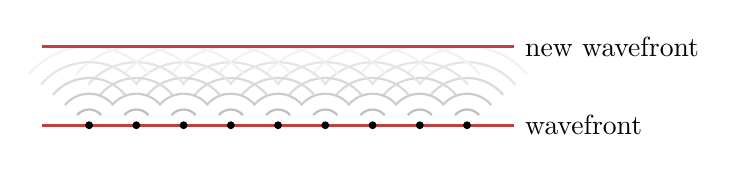
\begin{tikzpicture}
    \draw[very thick,gray!50!red] (0,0)--(6,0) node[right,black]{wavefront};
    \foreach \x in {5.4,4.8,...,.4}{
      \fill (\x,0) circle(.05);
      
      \begin{scope}[thick]
        \draw[gray!50] (\x,.2) arc (90:40:.2);
        \draw[gray!50] (\x,.2) arc (90:140:.2);
        \draw[gray!40] (\x,.4) arc (90:40:.4);
        \draw[gray!40] (\x,.4) arc (90:140:.4);
        \draw[gray!30] (\x,.6) arc (90:40:.6);
        \draw[gray!30] (\x,.6) arc (90:140:.6);
        \draw[gray!20] (\x,.8) arc (90:40:.8);
        \draw[gray!20] (\x,.8) arc (90:140:.8);
        \draw[gray!10] (\x, 1) arc (90:40:1);
        \draw[gray!10] (\x, 1) arc (90:140:1);
      \end{scope}
    }

    \draw[very thick,gray!50!red] (0,1)--(6,1)
    node[right,black]{new wavefront};

    \end{tikzpicture}
\end{figure}
%
%
%
%
%\section{Applying Huygens' Principle: Circular Wave}
%
%    \begin{itemize}
The same model can be used to predict the propagation of a circular  wavefront
%    \item<3->Again, each wavelet propagates radially outward at the same wave
%      speed
%    \item<4->The wavelets shows where the wavefront will be moved to
%      after $\Delta t$
%    \end{itemize}
%
\begin{figure}[ht]
  \centering
  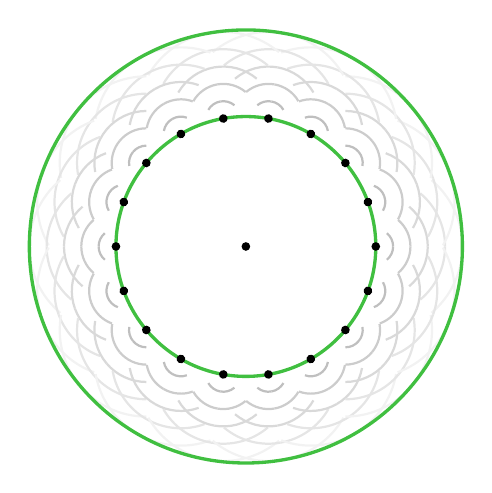
\begin{tikzpicture}[scale=1.1]
    \fill circle (.05);
    \draw[very thick,gray!50!green] circle(1.5);
    \foreach \theta in {0,20,...,359}{
      \begin{scope}[rotate=\theta]

        \fill (1.5,0) circle (.05);

        \draw[thick,gray!50] (1.7,0) arc (0:50:.2);
        \draw[thick,gray!50] (1.7,0) arc (0:-50:.2);
        \draw[thick,gray!40] (1.9,0) arc (0:50:.4);
        \draw[thick,gray!40] (1.9,0) arc (0:-50:.4);
        \draw[thick,gray!30] (2.1,0) arc (0:50:.6);
        \draw[thick,gray!30] (2.1,0) arc (0:-50:.6);
        \draw[thick,gray!20] (2.3,0) arc (0:50:.8);
        \draw[thick,gray!20] (2.3,0) arc (0:-50:.8);
        \draw[thick,gray!10] (2.5,0) arc (0:50:1);
        \draw[thick,gray!10] (2.5,0) arc (0:-50:1);
      \end{scope}
    }

    \draw[very thick,gray!50!green] circle (2.5);
    \end{tikzpicture}
\end{figure}

%
%
%
%
%\section{Reflection}
%
\section{Reflection of Light}

In the  \textbf{Law of Reflection}, the incident ray, the reflected ray, and
the normal to the surface of the mirror all lie in the same plane, and the
angle of reflection $\theta_r$ is  equal to the angle of incidence $\theta_1$:
\begin{equation}
  \boxed{\theta_r=\theta_1}
\end{equation}

%  \begin{center}
%    \pic{.65}{graphics/Types-of-reflection}
%  \end{center}
%
%
%
%
\begin{figure}[ht]
  \centering
  \pic{.5}{lightWaves/graphics/Lake-reflection}
\end{figure}
This photo of Lake Matheson shows specular reflection in the water of the
lake with reflected images of Aoraki/Mt Cook (left) and Mt Tasman (right).
The very still lake water provides a perfectly smooth surface for this to
occur.



\section{Refraction}

\textbf{Refraction} is the change in wave speed and direction when the wave
enters another medium with a different wave speed. When the wave enters the
medium at an angle, the change of wave speed causes
the wave to  change direction (e.g.\ from air to water, air to glass, glass to
air etc). The amount of bending depends on an optical property of the
two media, called the inndex of refraction.

%    \pic1{graphics/p023hqnk}
%  
%  \vspace{.2in}Refraction happens not only with light, we see the same
%  behaviour in ocean waves, when the wave travel from deeper water (faster
%  waves) to shallow depths.
%
%
%
%\section{Refraction of Light Through a Medium}
%  When light enters from one medium to another, it both reflects and refracts:
%  \begin{center}
%    \begin{tikzpicture}
%      \fill[lightgray] (-3,-2) rectangle (3,0);
%      \draw[thick] (-3,0)--(3,0);
%      \draw[red!80,very thick] (-2,2)--(0,0)--(1,-2)
%      node[above right=0,black]{Refraction};
%      \draw[red!80,very thick] (0,0)--(2,2) node[right=0,black]{Reflection};
%      \draw[dashed] (0,2)--(0,-2);
%      \draw[axes] (0,1) arc (90:135:1) node[midway,above]{$\theta_1$};
%      \draw[axes] (0,-1) arc (270:297:1) node[midway,below]{$\theta_2$};
%      \node[above] at (-2,0) {$n_1$};
%      \node[below] at (-2,0) {$n_2$};
%      \node[above] at (2,0) {$c_1$};
%      \node[below] at (2,0) {$c_2$};
%    \end{tikzpicture}
%  \end{center}
%  The reflection follows the law of reflection; the angle $\theta_2$ is
%  determined by Snell's law.



\subsection{Snell's Law}
\textbf{Snell's law}, also known as the \textbf{law of refraction}, relates the
indices of refraction $n$ of the two media to the directions of propagation
in terms of the angles to the normal. 
\begin{equation}
  \boxed{
    n_1\sin\theta_1=n_2\sin\theta_2
  }
  \label{eq:law-of-refraction}
\end{equation}
%  \begin{center}
%    \begin{tabular}{l|c|c}
%      \rowcolor{pink}
%      \textbf{Variable} & \textbf{Symbol} & \textbf{SI Unit}\\ \hline
%      Indices of refraction of the media & $n_1$, $n_2$ & (no units)\\
%      Incident angle of light   & $\theta_1$ & (no units)\\
%      Refraction angle of light & $\theta_2$ & (no units)
%    \end{tabular}
%  \end{center}
%
%
%
%
%\section{Refraction and Huygens' Principle}
%  
%    \pic1{graphics/huygen}
%    
%    We can explain the refraction phenomenon using Huygens' principle
%  
%
%
%
%
%

The \textbf{index of refraction}, or \textbf{refractive index}, of a material
($n$) is the ratio between the speed of light in vacuum ($c_0$) and the speed
of light in the medium ($c$):
%    or just the \textbf{index}.} ($n$) is the ratio between the
\begin{equation}
  \boxed{n=\frac{c_0}c=\frac{\lambda_0}\lambda}
\end{equation}
%
%  When light enters a medium, the \emph{frequency} remains constant (i.e.\ the
%  colour does not change), but since the speed changes, the \emph{wavelength}
%  will change, by applying $c=f\lambda$:
%    
%  \eq{-.1in}{
%    \boxed{\frac{n_1}{n_2}=\frac{\lambda_2}{\lambda_1}}
%  }


Indices of refraction are usually determined experimentally. Incides of some
common materials are shown in Table~\ref{tabl:index-of-refraction}. These are
typically the \emph{average values} that do not account for variations with
wavelength.

\begin{table}[ht]
  \centering
  \begin{tabular}{c|c||c|c}
    \rowcolor{pink}
    \textbf{Material} & $n$ & \textbf{Material} & $n$\\ \hline
    Vacuum           & 1     & Ethanol     & 1.362 \\
    Air     & \num{1.000277} & Glycerine   & 1.473 \\
    Water at \SI{20}\celsius & 1.33 & Ice  & 1.314 \\
    Carbon disulfide & 1.63  & Polystyrene & 1.59 \\
    Methylene iodide & 1.74  & Crown glass & 1.50 to 1.62 \\
    Diamond          & 2.417 & Flint glass & 1.57 to 1.75
  \end{tabular}
  \caption{Index of refraction of common materials}
  \label{tabl:index-of-refraction}
\end{table}
%which
%causes \emph{dispersion}.



\subsection{Total Internal Reflection}
When light is transmitted from a high index material to a lower index material
(i.e.\ $n_1>n_2$), Snell's law (Eq.~\ref{eq:law-of-refraction}) shows that the
angle of refraction $\theta_2$ is greater than the angle of incident $\theta_1$
(i.e.\ $\theta_2>\theta_1$), as shown in Figure~\ref{fig:no-tir}.

\begin{figure}[ht]
  \centering
  \begin{subfigure}[t]{.32\linewidth}
    \centering
    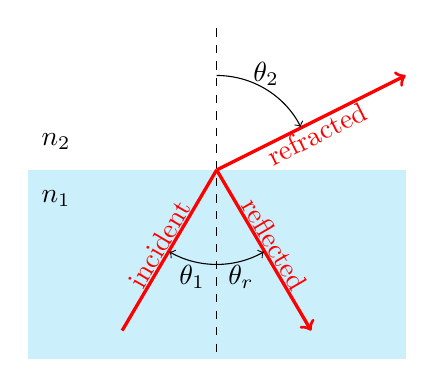
\begin{tikzpicture}[scale=1.2]
      \fill[color=cyan!20] rectangle (4,-2);
      \node at (.3,-.3) {$n_1$};
      \node at (.3,.3) {$n_2$};
      \draw[dashed] (2,1.5)--(2,-2);
      \begin{scope}[very thick,red]
        \draw (1,-1.7)--(2,0) node[sloped,midway,above=-3]{incident};
        \draw[->] (2,0)--(3,-1.7) node[sloped,midway,above=-3]{reflected};
        \draw[->] (2,0)--(4,1) node[sloped,midway,below=-3]{refracted};
      \end{scope}
      \draw[->] (2,-1) arc (270:240:1) node[midway,below=-2]{$\theta_1$};
      \draw[->] (2,-1) arc (270:300:1) node[midway,below=-2]{$\theta_r$};
      \draw[->] (2,1) arc (90:27:1) node[midway,above=-2]{$\theta_2$};
    \end{tikzpicture}
    \caption{Light transmits from high to low index material at small angle.}
    \label{fig:no-tir}
  \end{subfigure}
  \hspace{\stretch1}
  \begin{subfigure}[t]{.32\linewidth}
    \centering
    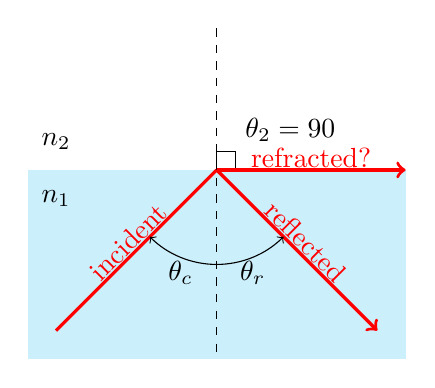
\begin{tikzpicture}[scale=1.2]
      \fill[color=cyan!20] rectangle (4,-2);
      \node at (.3,-.3) {$n_1$};
      \node at (.3,.3) {$n_2$};
      \draw[dashed] (2,1.5)--(2,-2);
      \draw (2,0) rectangle +(.2,.2) node[above right]{$\theta_2=\ang{90}$};
      \begin{scope}[very thick,red]
        \draw (.3,-1.7)--(2,0) node[sloped,midway,above=-3]{incident};
        \draw[->] (2,0)--(4,0) node[midway,above=-3]{refracted?};
        \draw[->] (2,0)--(3.7,-1.7) node[sloped,midway,above=-3]{reflected};
      \end{scope}
      \draw[->] (2,-1) arc (270:225:1) node[midway,below=-2]{$\theta_c$};
      \draw[->] (2,-1) arc (270:315:1) node[midway,below=-2]{$\theta_r$};
    \end{tikzpicture}
    \caption{At critical angle $\theta_1=\theta_c$, angle of refraction is
      \ang{90}}
    \label{fig:critical-angle}
  \end{subfigure}
  \hspace{\stretch1}
  \begin{subfigure}[t]{.32\linewidth}
    \centering
    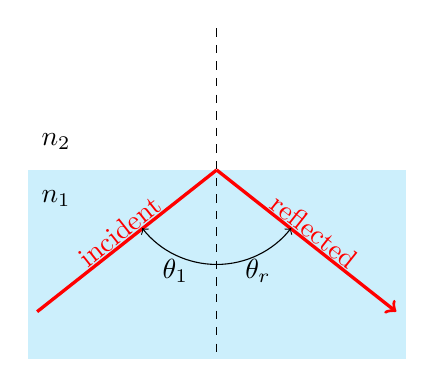
\begin{tikzpicture}[scale=1.2]
      \fill[color=cyan!20] rectangle (4,-2);
      \node at (.3,-.3) {$n_1$};
      \node at (.3,.3) {$n_2$};
      \draw[dashed] (2,1.5)--(2,-2);
      \begin{scope}[very thick,red]    
        \draw (.1,-1.5)--(2,0) node[sloped,midway,above=-3]{incident};
        \draw[->] (2,0)--(3.9,-1.5) node[sloped,midway,above=-3]{reflected};
      \end{scope}
      \draw[->] (2,-1) arc (270:218:1) node[midway,below=-2]{$\theta_1$};
      \draw[->] (2,-1) arc (270:322:1) node[midway,below=-2]{$\theta_r$};
    \end{tikzpicture}
    \caption{Beyond the critical angle, all light is reflected back}
    \label{fig:TIR}
  \end{subfigure}
\end{figure}
As the angle of incident increases, the angle of refraction will reach \ang{90}
first. When the angle of refraction is at \ang{90}, the angle of incident is
called the \textbf{critical angle} $\theta_c$, as shown in
Figure~\ref{fig:critical-angle}. Refracted light can still be observed
\emph{at} the interface, but only if the interface is perfectly smooth. We can
calculate the critical angle by setting $\theta_2=\ang{90}$ (i.e.\
$\sin\theta_2=1$) and solving for $\theta_1$:
\begin{equation}
  \boxed{
    \theta_c=\sin^{-1}\left(\frac{n_2}{n_1}\right)
  }
\end{equation}
Critical angle $\theta_c$ for water-air interface ($n_\text{air}=1$ and
$n_\text{water}=1.33$) is \ang{48.6}.

When the angle of incident is greater than the critical angle (i.e.\
$\theta_1>\theta_c$), Snell's law fails, because $\sin\theta_2$ cannot be
greater than 1. At this time, \textbf{total internal reflection} occurs. All
the incident light onto the interface is reflected back into the first medium,
as shown in Figure~\ref{fig:TIR}. Obviously, total internal reflection can only
occur when light travels from high index material towards a lower index
material, $n_1>n_2$.



\section{Dispersion}
%
%\section{Colour of Light and Wavelength}
%  Human eyes perceive different frequencies of light as different colours.
%  The visible spectrum of light correspond to wavelengths\footnote{In a vacuum}
%  approximately from \SI{750}{\nano\metre} (\textcolor{red}{red}) to
%  \SI{380}{\nano\metre} (\textcolor{blue!70!black}{violet}):
%
%  \vspace{-.2in}\begin{center}
%    \pic{.4}{graphics/visiblespectrum}
%  \end{center}
%  The ``colour'' of the light depends on its frequency\footnote{Although it is
%    usually expressed as the wavelength of the light in a vacuum}
%
%
%
%
%\section{Dispersion of Light Through Refraction}
% 
%    \pic{1.1}{graphics/white-light-split-into-colours-by-a-prism-pasieka}
%    
\begin{itemize}
\item\textbf{White light} is a light that is composed of multiple colours
  in the visible-light spectrum
\item When white light passes through a prism it is separated into
  different colours
\item This is because the refractive index $n$ varies slightly with
  wavelengths (without this variation, we'd never see a rainbow)
\item The phenomenon is of splitting light into its component colours is
  called \textbf{dispersion}
\end{itemize}
  




%\section{Wavelength Dependency of Index of Refraction}
%  \centering
%  \pic{.5}{graphics/Dispersion-curve}
%
%
%
%
%\section{Chromatic Aberration}
%  When looking at an image through a cheap binocular, magnifying glass, or
%  telescope, we see the edges of images blurred with a rainbow-coloured edge:
%  \begin{center}
%    \pic{.45}{graphics/choosing03-pic002}
%  \end{center}
%  \textbf{Chromatic aberration} occurs even with high-quality camera lenses,
%  particularly with wide-angle lenses where light has to refract from high
%  angles towards the camera sensor/film
%
%
%
%
%\section{Chromatic Aberration}
%  The reason that chromatic aberration happens is the same reason that prisms
%  work: through dispersion of light
%  \begin{center}
%    \pic{.4}{graphics/chromatic-aberration-feature-image}
%  \end{center}
%  The focal lengths for different frequencies (colour) of light are different,
%  thus blurring the image. So how do we fix it?
%
%
%
%
%\section{Chromatic Aberration: Camera Lens Design}
%  By arranging different lenses of different materials and geometries, we can
%  correct for the chromatic aberration.
%  \begin{center}
%    \pic{.4}{graphics/Apochromatic-Lens}
%  \end{center}
%  Lens design is a closely guarded secret by camera companies. Shape of the
%  lens, material and coating are all factors. A ``lens'' on a DSLR camera can
%  have up to 30 lens ``elements''
